\chapter{Elicited Monotonic Fairness} \label{ch:SoftMonoFair}

\section{Overview}

    Monotonicity as discussed in Chapter \ref{ch:MonoFair} requires that individual attributes can be assigned a monotonic relationship with the outcome, but does not account for intuitive monotonicity which might occur across combinations of attributes.  For instance, consider the situation where two defendants are otherwise identical except that the first has committed ten more felonies and the second has committed one more misdemeanor; clearly, the first should be ranked as more likely to re-offend, but the two are incomparable according to these strict monotonicity rules.  
    
    In addition, such strict interpretation of monotonicity prevents comparison between individuals with non-identical covariates on non-monotonic axes.  For example, if two defendants are 30 and 31 years old, they are incomparable regardless of their other records.
    
    This section explores a methodology for eliciting such non-axial monotonicity based on surveying arbiters, which may or may not be fair in their judgments, and using those responses to regularize a classifier.  The input of the arbiters is motivated as preventing intuitive resentment. 

\section{Background}\label{sec:softmono_bg}
    
    We assume that the reader is familiar with the definitions and concepts in Sections \ref{sec:monofair_intro} and \ref{sec:monofair_background}.  We wish to extend the concept of \emph{non-protected attribute resentment} (Def. \ref{def:ScoreResentment}) to widen the comparisons which can be made when defining what is a ``better" $X_u$.
    
    At its core, the problem to be addressed is that an individual will have resentment toward others if the individual feels the others received better treatment despite not being as deserving.  Modeling each individual's views on relative treatment would be undesirable since we would like a rule which applies evenly to all individuals; we instead aim to learn a ranking function over individuals which can be used universally.  
    
    We propose to learn such a function by querying a set of arbiters by presenting pairs of non-protected attribute sets and asking for a judgment as to what the fair relative treatment of the pair would be. Once collected, these sample can be used to learn a \emph{preference function} over pairs of non-protected attributes which can be used to regularize the prediction function to prevent individual resentment while still providing accurate prediction that, optionally, also protects against group-level unfairness.

    This is not the first work to incorporate the idea of utilizing arbiter queries in the area of fairness.  The original definition of individual fairness given by Dwork \cite{dwork2012fairness} requires specificying a distance metric over attributes which can bound the difference in treatment, i.e. $D\left(f(X_i), f(X_j)\right) \le \kappa d(X_i, X_j)$.  Ilvento\cite{ilvento2019metric} and other recent works \cite{jung2019eliciting,lahoti2019operationalizing,wang2019empirical} approach the problem of operationalizing an individual fairness distance metric by polling arbiters on which pairs of individuals can be considered similar.  Wang et al.\cite{wang2019empirical} similarly collect actual survey data and evaluate a variety of models to interpret such data.  None of these approaches tackle the problem of dissimilar treatment, i.e. when an arbiter decides that two individuals should receive different predictions, especially the asymmetric case when arbiters indicate that one individual should receive a specifically more favorable or less favorable outcome than the other.
    
    Models which are designed to identify the relative values of pairs can generally be classified as preference learning models\cite{peters2018scalable} \guy{Flesh this out.}
    

\section{Model}\label{sec:softmono_model}

    Let $X^{obs}$, $Y^{obs}$, and $A^{obs}$ be the non-protected attributes, observed binary outcomes $\in \{0, 1\}$, and protected attributes for some set of $n$ individuals.  Using $i, j \in {1 \ldots n}^2$, we can construct pairings from the observed data, and we introduce an auxiliary variable,
    $$ Z_{ij}^{obs} = \left\{ \begin{array}{l c l}
        1 & \mbox{if} & Y_i^{obs} = 1 \mbox{~and~} Y_j^{obs} = 0 \\
        2 & \mbox{if} & Y_i^{obs} = 0 \mbox{~and~} Y_j^{obs} = 1 \\
        3 & \mbox{if} & Y_i^{obs} = Y_j^{obs}
    \end{array}\right. .$$
    
    The crux of this model is moving from optimizing for the direct prediction of outcomes encompassed by $Y$ to optimizing the relative outcomes encompassed by $Z$.  Similarly, when codifying our survey results When we survey our fairness arbiters, we ask them to evaluate whether one individual is more likely ($Z = 1$), less likely ($Z = 2$) or similarly likely ($Z = 3$) than another specific individual to have $Y = 1$.
    
    We can then define a single loss function which incorporates both data sources:
    $$ \mathcal{L}_Z = \sum\limits_{i, j \in \mathcal{O} + \mathcal{S}} \left(\begin{array}{l} 
        \mathbf{1}_{Z_{ij} = 1} ~ \hat{p}_i (1 - \hat{p}_j) ~ + \\
        \mathbf{1}_{Z_{ij} = 2} ~ (1 - \hat{p}_i) \hat{p}_j ~ + \\
        \mathbf{1}_{Z_{ij} = 3} ~ \left(\hat{p}_i \hat{p}_j + (1 - \hat{p}_i)(1 - \hat{p}_j) \right)
    \end{array}\right), \label{eq:sm_pairwise_loss}$$
    
    letting $\mathcal{O}$ denote the set of observed pairs and $\mathcal{S}$ denote the set of surveyed pairs.  Note that the $\mathcal{S}$ may be either the whole set $\{1 \ldots N\}^2$ or a sample of the set.  $\mathcal{O} \cap \mathcal{S} = \mathcal{S}$ if $\mathcal{O}$ is the whole space, and may be a subset or empty set if $\mathcal{O}$ is a sample of the pairwise comparisons.

\section{Experiments}\label{sec:softmono_experiments}

    We demonstrate the use of the above pairwise loss on two datasets.  First, we consider a synthetic experiment where the true probability $\Pr(Y_i = 1 | X_i)$ is known and we attempt to recover that probability using a simple feedforward neural network, as described in Sections \ref{sec:intro_nns} and \ref{sec:monofair_experiments}, trained to minimize \ref{eq:sm_pairwise_loss}.  
    
    Second, we consider the COMPAS dataset, and utilize human survey responses and attempt to learn a network with a conditional prediction structure which allows for post-hoc compromise between fairness loss and prediction accuracy.  We set $X_{c}$ to 0 when using pairs from observed data and to 1 when using pairs from surveyed data.

    \subsection{Synthetic - Proof of balancing objectives}
    
        We begin with a synthetic experiment where the ground truth.  We have an individual set of attributes $X_i \sim N(0, 1)^2$, and two weight vectors,  $\beta_{obs} = [0.9, 1.1]$ and $\beta_{sur} = [1.1, 0.9]$, which describe the relationship between $X$ and,respectively,  $Z_{ij}^{obs}$ (via $Y_{i}^{obs}$) and $Z_{ij}^{sur}$.  We set $P_i^{obs} = 1 / (1 + \exp{-X_i \beta^{obs} - 1})$, sample $Y_i \sim \mbox{Bernoulli}(P_i^{obs})$, and set $Z_{ij}^{obs}$ as defined as above.  We set $Z_{ij}^{sur}$ according to:
            $$ Z_{ij}^{sur} = \left\{ \begin{array}{lll}
                    1 & \mbox{if} & X_{i}\beta^{sur} > X_{j}\beta^{sur} + 0.25\\
                    2 & \mbox{if} & X_{j}\beta^{sur} > X_{i}\beta^{sur} + 0.25 \\
                    3 & \mbox{if} & | X_{i}\beta^{sur} - X_{j}\beta^{sur} | < 0.25
                \end{array} \right. .$$
        We sample 1,000 training examples of $Z_{ij}^{obs}$ and 200 examples of $Z_{ij}^{sur}$, and evaluate losses on the same number identically distributed held out samples.  We trained using a small neural network of three hidden layes of width three and a $\tanh$ activation function.
        
        First, we wish to establish that the pairwise loss defined above is competent to estimate the probability function underlying probability function when $X_c = 0$ i.e. when attempting to predict based purely on the observed outcomes via the $Z_{ij}$ pairs.  In Figure \ref{fig:sm_synthetic_p_fit}, we show experimentally that $\hat{P}_i$ is accurate to within the limit of sampling error and (intentional) model misspecification.
        
        \begin{figure}
            \centering
            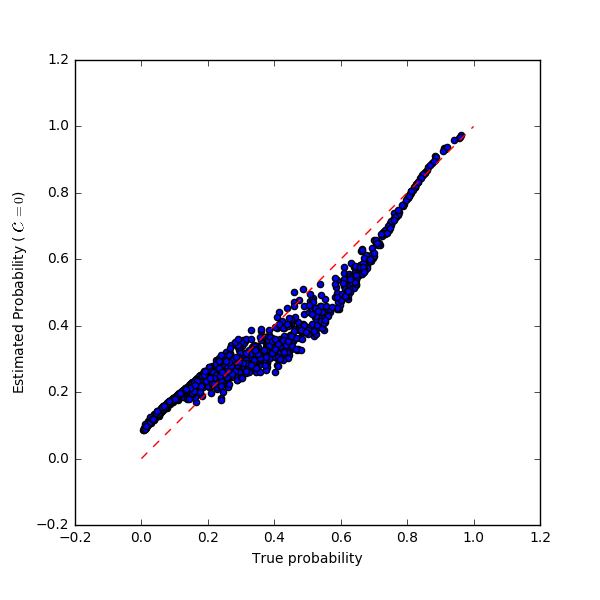
\includegraphics{fig_softmono/synthetic_p_fit.png}
            \caption{The model estimated probability of $\Pr(Y_i = 1 | X_i, X_c = 0)$ versus the ground truth probabilities, with 1:1 line.}
            \label{fig:sm_synthetic_p_fit}
        \end{figure}
        
        Second, we wish to assess whether the model is able to interpolate via $X_c$ between it's dual goals of predicting $\hat{Y}_i$ while adhering to the surveyed $Z_{ij}^{sur}$ pairs.  The trend of $Z_{ij}^{sur}$ is exactly as expected; lowest when $X_c = 0$ and gradually increasing to a maximum when $X_c = 1$.  The behavior of $Z_{ij}^{sur}$ is less intuitive; it is highest when $X_c = 0$, but many random fits have an local minimum loss with $X_c < 1$.  This is explained by the relatively small sample ($n^{sur} = 200$) leading to overfitting even in this modest network, and by $\mathcal{L}_Z^{obs}$ providing regularization which improves out-of-sample performance.  We also, when examining the joint loss values available, that the models fits form appropriate trade off functions for performance, with reduction of one loss coming at the cost of increase of the other. 
        
        \begin{figure}
            \centering
            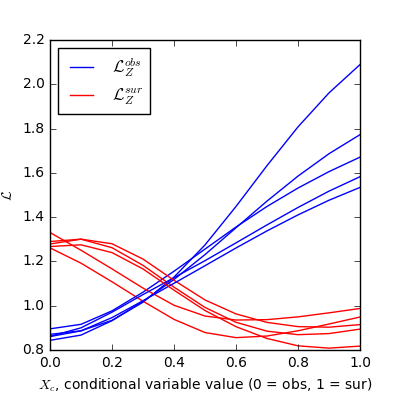
\includegraphics[width=0.45\textwidth]{fig_softmono/synthetic_loss.png}
            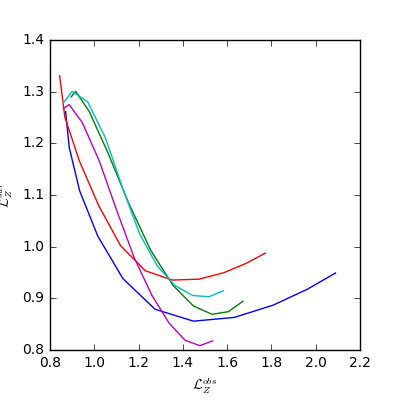
\includegraphics[width=0.45\textwidth]{fig_softmono/synthetic_loss_tradeoff.png}
            \caption{
                Model losses as a function of conditional variable ($X_c$) setting over 5 experiments with random initializations.  Left: losses as a function of $X_c$, with $\mathcal{L}_Z^{obs}$ in blue and $\mathcal{L}_Z^{sur}$ in red.  Right: parametric plot of $\mathcal{L}_Z^{sur}$ as a function of $\mathcal{L}_Z^{obs}$.
            }
            \label{fig:sm_synthetic_losses}
        \end{figure}
        
    \subsection{COMPAS}
    
        We augment the COMPAS dataset described in Section \ref{sec:monofair_datasets} in two ways: we add a feature for whether the current charge is violent, and we collect survey data to on random pairs and the possible ordering of their outcomes.
        
        The first augmentation was made by survey.  Five volunteers were each presented 100 independent random pairings of non-protected attributes, labeled ``Individual A" and ``Individual B", and asked to provide one of four ratings:
        \begin{itemize}
            \item ``A is at least as likely to (re)offend" ($Z = 1$)
            \item ``B is at least as likely to (re)offend" ($Z = 2$)
            \item ``A and B are similarly likely to (re)offend" ($Z = 3$)
            \item ``No preference / any of the others are fair"
        \end{itemize}
        The full survey instructions are presented in the appendix.  Seventeen responses indicating no preference were discarded, leaving 298 dissimilar responses ($Z \in \{1, 2\}$) and 185 similar responses ($Z = 3$).

        Second, in adding the feature for violence of the current charge, we utilized the classification system described by ProPublica and based on the US Department of Justice's definition of a violent crime: ``murder and nonnegligent manslaughter, forcible rape, robbery, and aggravated assault."  With this feature added, the non-protected attributes are age, (adult) priors count, juvenile prior felony count, juvenile prior misdemeanor count, juvenile prior other counts, arrest charge degree (felony or misdemeanor), and whether the arrest charge is violent.  The protected attributes are race, classified as Caucasian, African American, or Other (comprising what the dataset labels as Other, Hispanic, Native American, and Asian), and Sex, classified as Male or Female.
        
        We feed the neural network an additional input: whether the data point is from the observed data or the surveyed data.  This design allows us to a tune a prediction continuously from being based entirely on real data without concern for agreeing with intuitive resentment and being based entirely on the survey data at the expense of predictive accuracy.
        
        For fairness loss, we chose to evaluate equality of odds, which requires that the prediction is independent of the protected attributes conditioned on the true outcome, i.e.
        $$ \Pr(\hat{Y} = 1 | A = a, Y = y) = \Pr(\hat{Y} = 1 | A = a', Y = y) \forall a, a', y .$$
        
        We express this is a differentiable loss as 
        $$
            \mathcal{L}_F = \sum\limits_{y} \sum\limits_{a} \left( \bar{\hat{y}}_{ay} - \bar{\hat{y}}_{\cdot y} \right)^2
        $$
        where $\bar{\hat{y}}_{ay} = \sum_{i: A_i = a, Y_i = y}(\hat{Y}_i) / n_{ay}$, i.e. the average prediction individuals of each protected attribute set and true outcome, and $\bar{\hat{y}}_{\cdot y} = \sum_{i: Y_i = y}(\hat{Y}_i) / n_{\cdot y}$, i.e. the average prediction for individuals of that true outcome.
        
        \begin{figure}
            \centering
            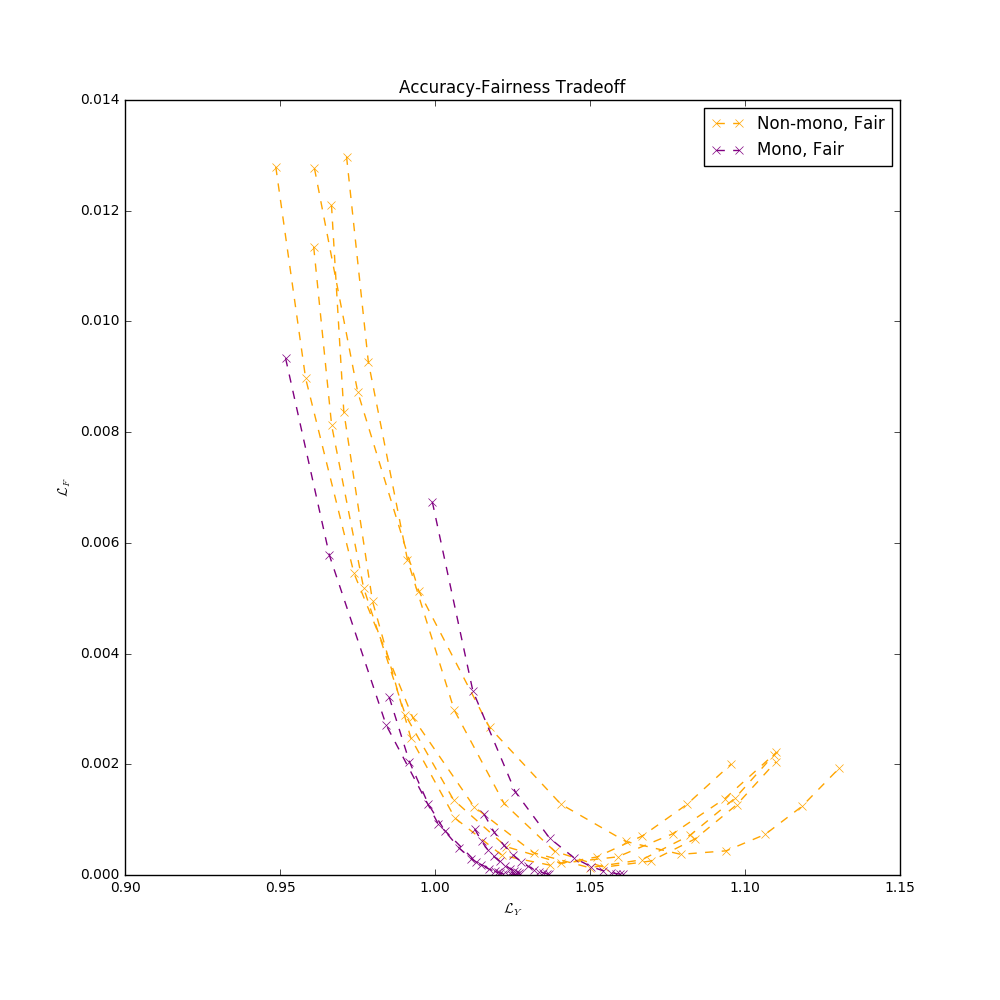
\includegraphics[width=\textwidth]{fig_softmono/compas_tradeoffs_fair.png}
            \caption{Fairness-Accuracy tradeoff for fair models}
            \label{fig:sm_compas_tradeoffs}
        \end{figure}
        
        \begin{figure}
            \centering
            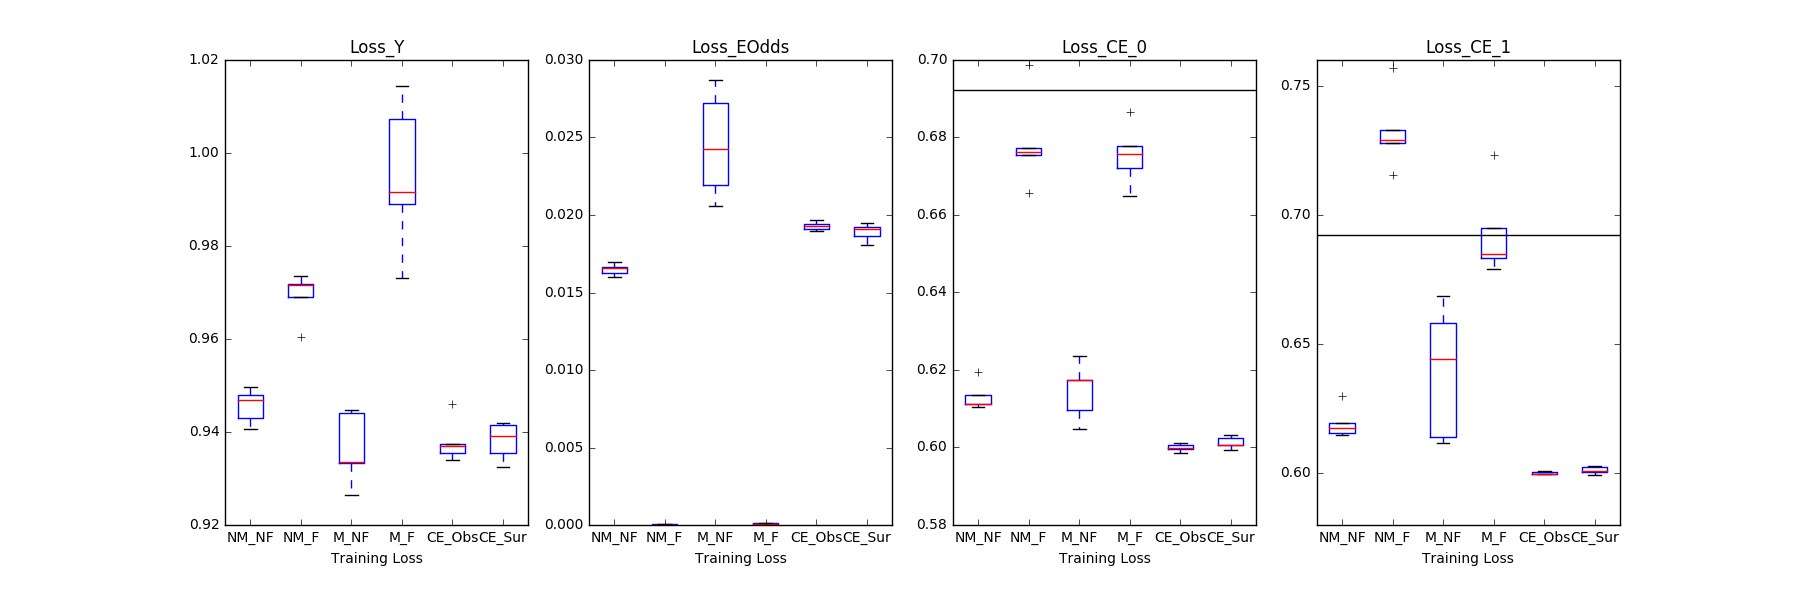
\includegraphics[width=\textwidth]{fig_softmono/compas_boxplot.png}
            \caption{Boxplots of model losses based on training regime}
            \label{fig:sm_compas_boxplots}
        \end{figure}
        

% \section{Discussion}\label{sec:softmono_discussion}
    
%     TBD
